\newpage

\section{机械结构设计}

\subsection{总体结构设计}

主要设计目标是设计一个自动车通用底盘:以“通用化”为核心特点,底盘被封装在一个扁平的车身中,未来将可以依据不同造型与功能需求,在云台位置搭载不同功能模块,如物流、快递、清扫、运输、甚至军警用特种装备等模块,成为适用于特定场景下各种功能的无人驾驶车辆。目前设计以搭载ZED双目摄像头,用于室内/外SLAM作为本设计的蓝本。

基本要求如下:长宽尺寸尺寸不超过 $ 1000mm \times 1000mm $的尺寸,实现简易有效的避震设计,传感器选用上采取模块化方法,并尽可能选取标准件,保障整体系统稳定性的实现。

首先将本机器人的命名确定为AtomIC(自动车通用底盘, \emph{Autonomous vehicle universal chassis})

因此我们由整体和功能的角度,结合抽象方法和模型方法的特征从总功能输入输出转换关系图,然后再建立分功能的结构简图,先画出最基本的功能即执行功能再画出他的输入和输出,最后图中各种流借助不同线型完成下方所示黑箱图。

\begin{figure}[htbp]
	\centering
	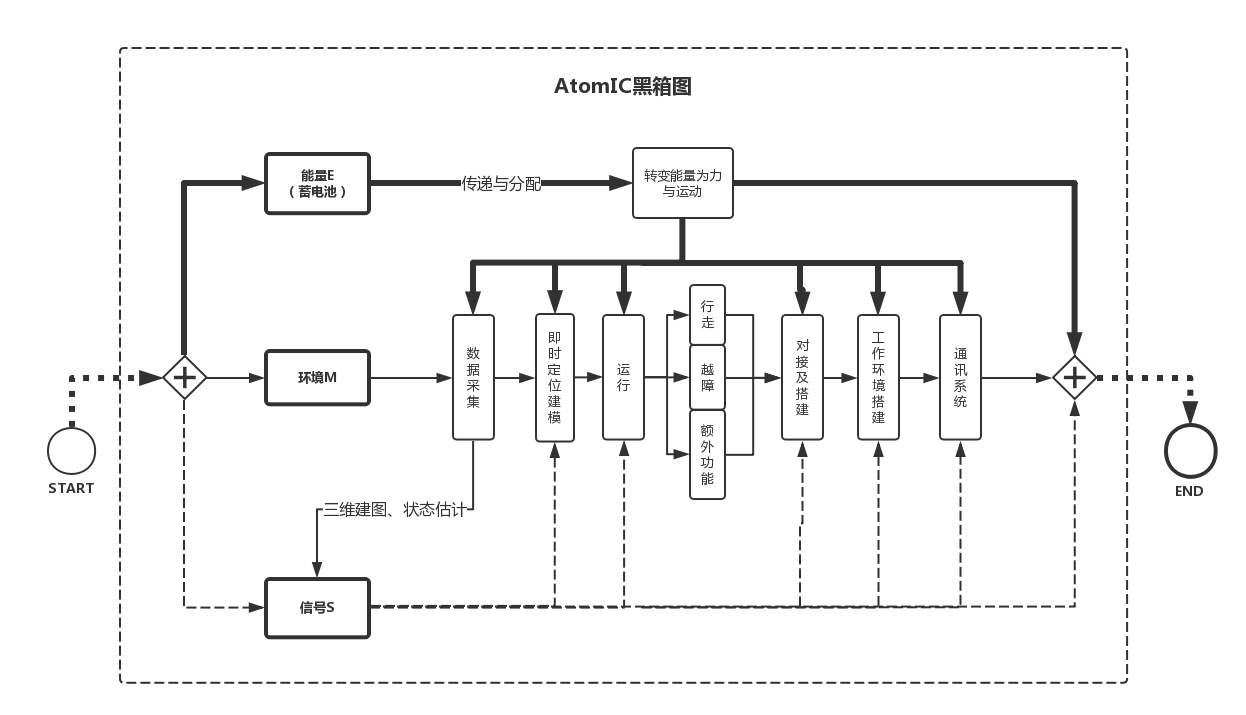
\includegraphics[width = 0.75\textwidth]{fig/hxt.png}
	\caption{功能黑箱图}
	\label{hxt}
\end{figure}

因此本无人车通用底盘的机械结构主要分为\textbf{车身主体,避震悬架,云台结构、电子元件保护结构以及其他结构}等结构,形态学矩阵如下图。

\begin{figure}[htbp]
	\centering
	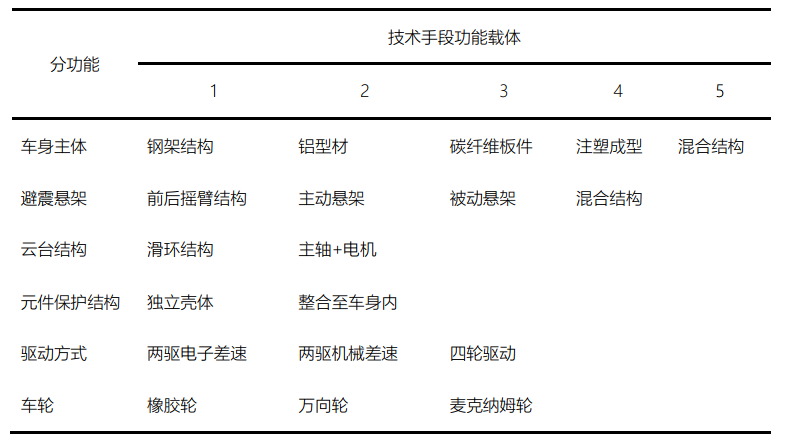
\includegraphics[width = 0.7\textwidth]{fig/xtxjz.png}
	\caption{形态学矩阵}
	\label{xtxjz}
\end{figure}

一共有多少$ 5 \times 4 \times 2 \times 2 \times 3 \times 3 =720 $种,而最终。在多种方案选择下,我们选取来这种"钢铝车身+碳纤维,被动避震,滑环结构、独立壳体、四轮驱动麦克纳姆轮"的方案。主要的优点如下:

\begin{enumerate}
	\item 对于车身主体方面,我们采用钢铝车身加工件与型材配合碳纤维主板的结构,这样的结构在保证强度的同时能够一定程度上保证轻量化与高效化;
	\item 被动避震、滑环结构的选择主要考虑是AtomIC平台主要应用于控制算法等相关云台模块的实现,在保证稳定耐用的前提下保证经济;
	\item 对于四轮驱动麦克纳姆轮的选择,这两者在目前已有很多成熟可靠的方案,并且四轮驱动和麦克纳姆轮在狭小空间与特定场景操作灵活并且具有可拓展性。
	
\end{enumerate}

以下就具体的机械结构进行说明与分析。

\subsection{细节模块选型设计}

\subsubsection{驱动轮选择}

在竞赛机器人和特殊工种机器人中,全向移动经常是一个必需的功能。「全向移动」意味着可以在平面内做出任意方向平移同时自转的动作。为了实现全向移动,一般机器人会使用「全向轮」(Omni Wheel)或「麦克纳姆轮」(Mecanum Wheel)这两种特殊轮子。

全向轮与麦克纳姆轮的共同点在于他们都由两大部分组成:轮毂和辊子(roller)。轮毂是整个轮子的主体支架,辊子则是安装在轮毂上的鼓状物。全向轮的轮毂轴与辊子转轴相互垂直,而麦克纳姆轮的轮毂轴与辊子转轴呈 45° 角。理论上,这个夹角可以是任意值,根据不同的夹角可以制作出不同的轮子,但最常用的还是这两种。两者如下图所示,

\begin{figure}[htbp]
	\centering
	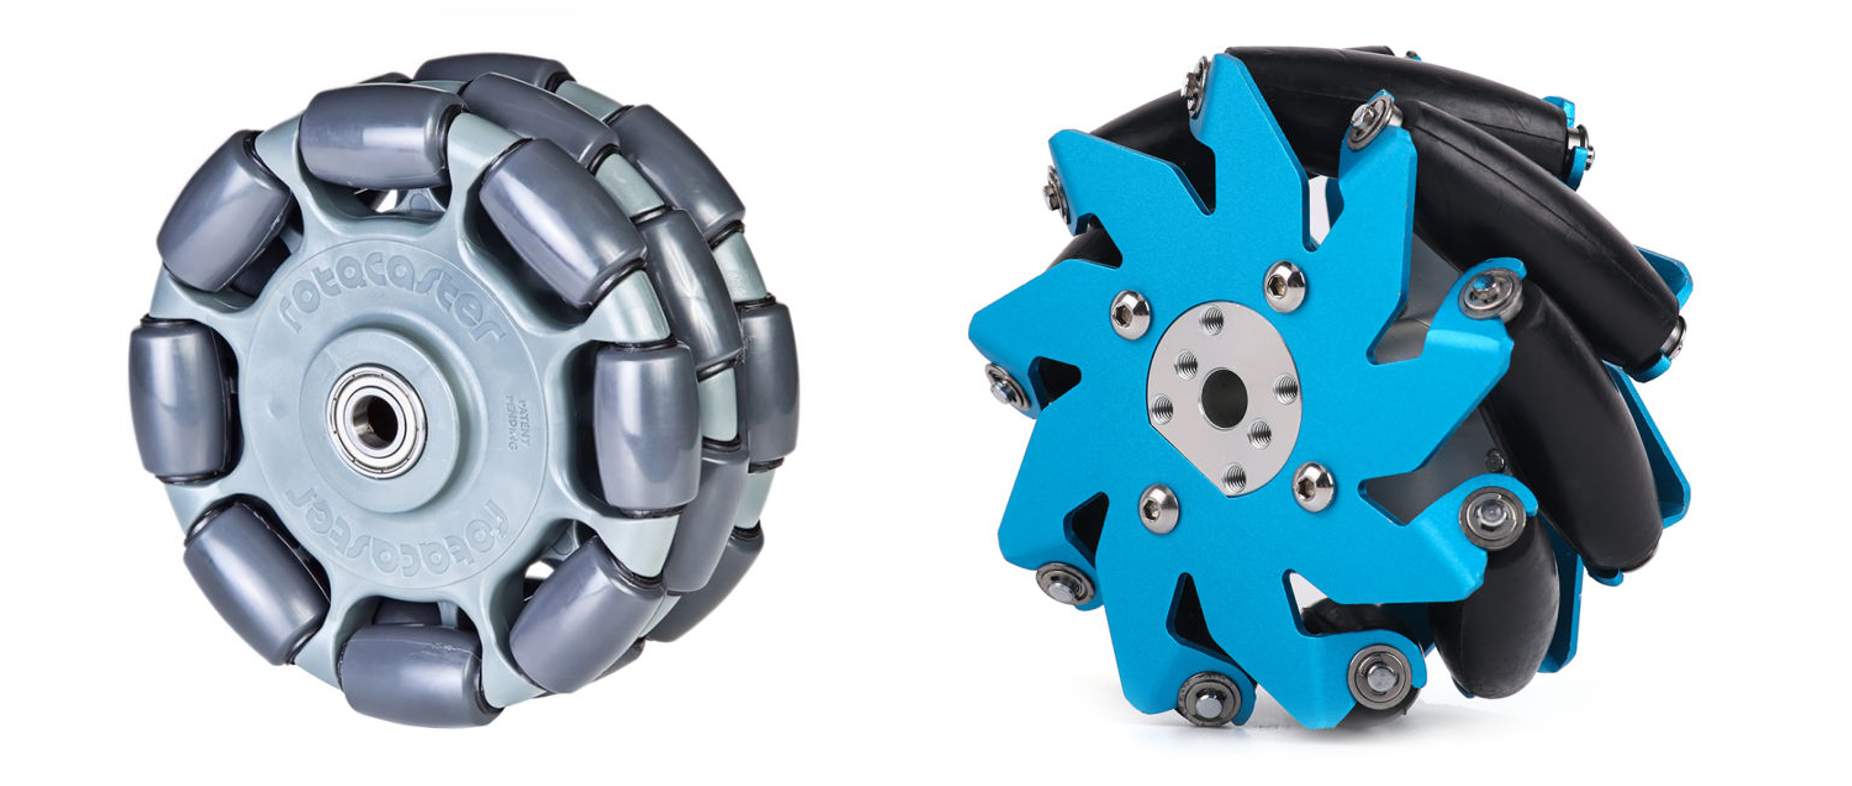
\includegraphics[width = 0.6\textwidth]{fig/qxlml.png}
	\caption{全向轮(左)和麦克纳姆轮(右)}
	\label{qxlml}
\end{figure}

近年来,麦克纳姆轮的应用逐渐增多,特别是在 RoboMaster、FRC 等机器人赛事上。这是因为麦克纳姆轮可以像传统轮子一样,安装在相互平行的轴上。而若想使用全向轮完成类似的功能,几个轮毂轴之间的角度就必须是 60°,90° 或 120° 等角度,这样的角度生产和制造起来比较麻烦。所以许多工业全向移动平台都是使用麦克纳姆轮而不是全向轮,因此麦克纳姆轮也是本报告的选择。

\subsubsection{底盘机构设计}

本次设计的底盘主要包括轮组装配及配合的顶板、 底板两部分。其中顶板、底板为配合四个轮组装配体的设计而得, 轮组装配体是本次设计的重点。 左右前后四个轮组装配体的互相对称以及齿轮传动的使用,提高空间利用效率,提高整体底板的机动性与抗击重载的稳定性。 以下是对轮组装配体部分的具体介绍:

在机械零件具体建模之前,对于所需功能尺寸进行预先设计。 考虑到避震器的正常工作长度区间在 65 到 85 mm 之间,使用 Solidworks 画出可变尺寸的草图, 就轮组装配体各个部分进行微调,以保证整体在正常范围内工作,提高了机构的可行性,为后续具体建模奠定了基础。

\begin{figure}[htbp]
	\centering
	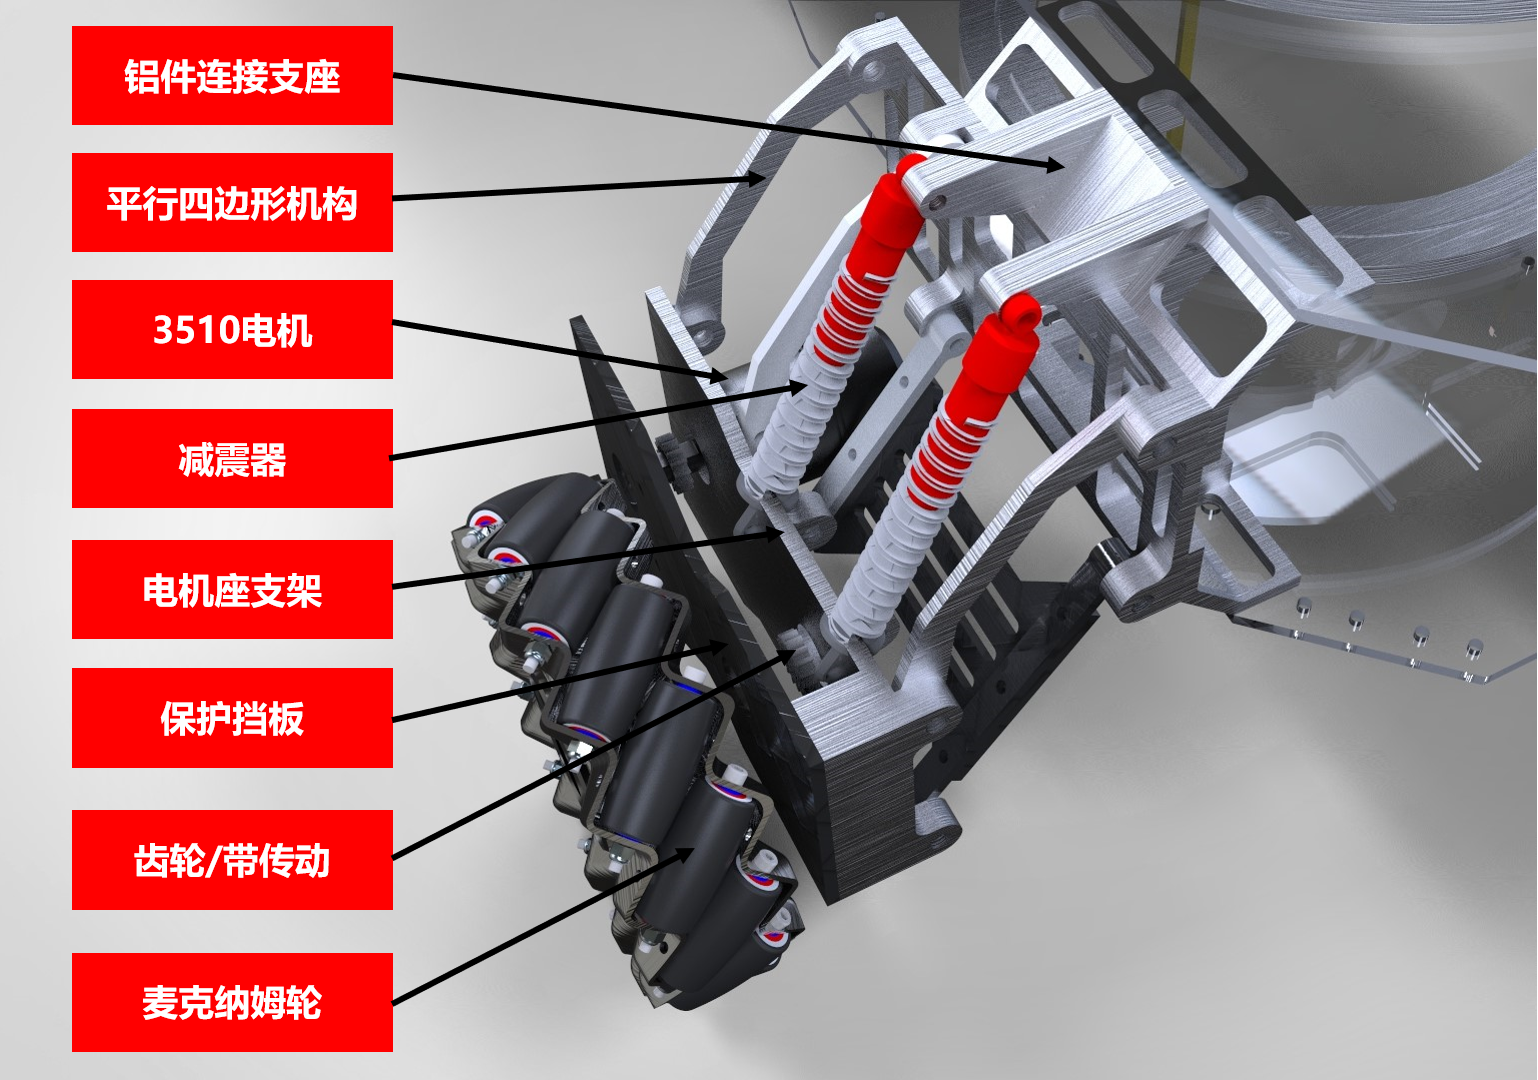
\includegraphics[width = 0.6\textwidth]{fig/dplb.png}
	\caption{底盘避震机构}
	\label{dplb}
\end{figure}

轮边装配体包括了平行四边机架和狗骨连轴传动机构两个部分。平行四边机架主要由上连杆、 下连杆,连板以及避震筒组成。 上连杆由中间螺柱加两端关节关节轴承, 上下分别用塞打螺丝固定在电机顶板及前部轴座上, 下连杆及连板由塞打螺丝及两个深沟球轴承固定在电机顶板及前部轴座上。 电机顶板、 底板分别由螺纹连接件固定在上图中所示的顶板、底板上。避震器安装在下连杆及避震器固定板上。 整体机架采用平行四边形连杆结构, 保证了麦克纳姆轮在各种工况下保持垂直与地面接触状态。 避震器的设计使用,将提高了整体小车的抗震性与稳定性。

同步轮传动机构主要由同步带、同步齿轮组成。同步轮传动主要由电机支座和保护板之间。同步轮的选用,提高了轮边轴系的自由度与稳定性, 方便了电机与避震器的布置设计。

\subsubsection{云台机构设计}

\begin{figure}[htbp]
	\centering
	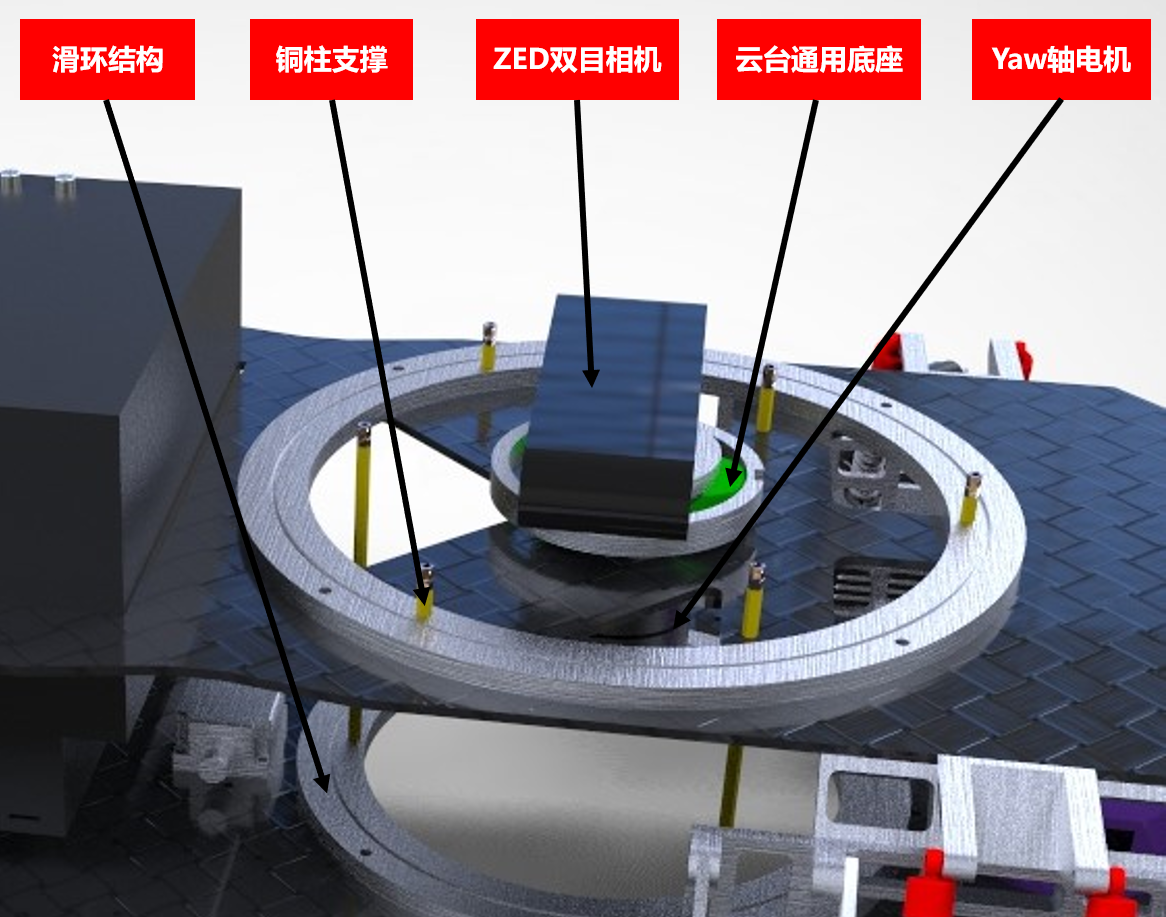
\includegraphics[width = 0.7\textwidth]{fig/ytjg.png}
	\caption{云台滑环机构}
	\label{ytjg}
\end{figure}

云台机构主要包括了滑环机构与通用连接支架两个部分。滑环机构主要由上滑环与中间铜柱支撑组成。云台采用结构, 保证了整车底盘可以实现不同功能的适配与完善,在保证经济适用的同时兼具稳定。

通用连接支架目前所安装设计部件为ZED双目摄像头,通过底板的优化设计,可以实现在统一安装支架上不同云台拓展部件的重复使用。
\\

\subsubsection{其他结构设计}

在整车其他部分,我还考虑到电池与相关处理器封装的布置。对于电池,初步想法是采用DJI智能保护电池,易充易换,且续航足够半天左右的实验时间,此外,双电池架设计,保证实车电源部件的冗余度与稳定,避免因为没电而在实验过程中断。未来预期的想法是将电池整合至车身隔板处,保证美观性并且避免因为雨雪天气带来的隐患。具体布置可见下图:

\begin{figure}[htbp]
	\centering
	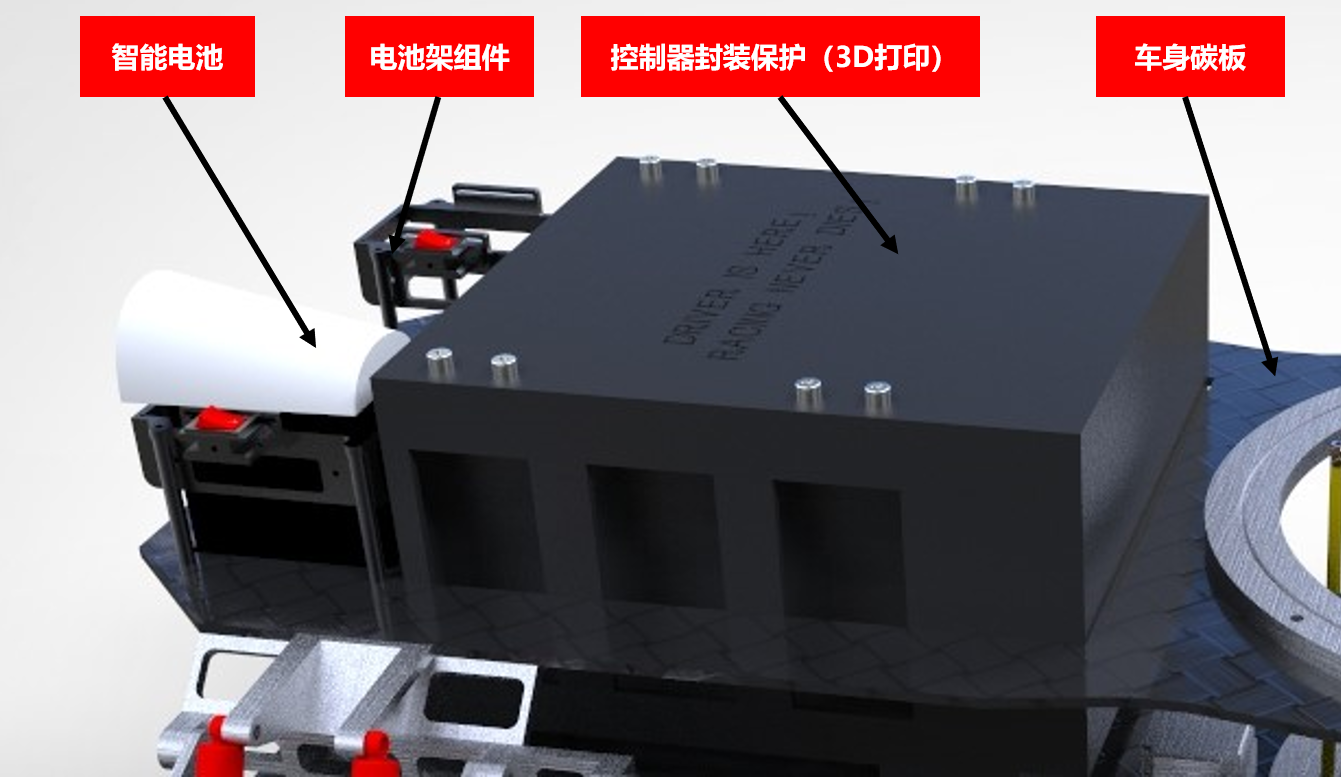
\includegraphics[width = 0.8\textwidth]{fig/qtjg.png}
	\caption{其他结构}
	\label{qtjg}
\end{figure}

此外,在处理器封装方面,目前在上下车板之间预留一定空间作为整个处理器封装的限位,整体考虑采用PC/尼龙打印或机加工工艺,保证AtomIC面对不同应用场景是具有较大的灵活性,此外,处理器必要的镂空与防水设计可以保证在程序烧录、数据读取的同时保证整体系统稳定可靠。

主板应该是安装零件最多的一个载体,上面包括云台、电池、前桥、妙算等重要部分,是最重要的一个零件。在设计主板形状时考虑两点因素,一个是受力。由前轮的支持力传来的力矩全部加在主板和轴承座的链接部位,这是整车最脆弱的地方。因此在连接部位的附近不可加减重孔,板材的厚度也要慎重考虑。二是装配的方便性。为此没有把yaw轴电机直接安装再主板上,而是专门做了一块电机安装板,一方面这样可以使云台整体拆装,与底盘分离。

\subsection{AtomIC平台设计总结}

\subsubsection{AtomIC平台最终设计}

以上是对一些重要结构的设计思路和一些重要零件进行简要的介绍。本设计参考RoboMaster17英雄底盘设计方案,所设计出的第一版AtomIC平台。平台保留四轮独立悬挂,采用前后轮独立悬挂的方案,选用适配弹簧结构,新的底盘在稳定性和性能上都有了极大的突破。下图为最终结构模块示意。

\begin{figure}[htbp]
	\centering
	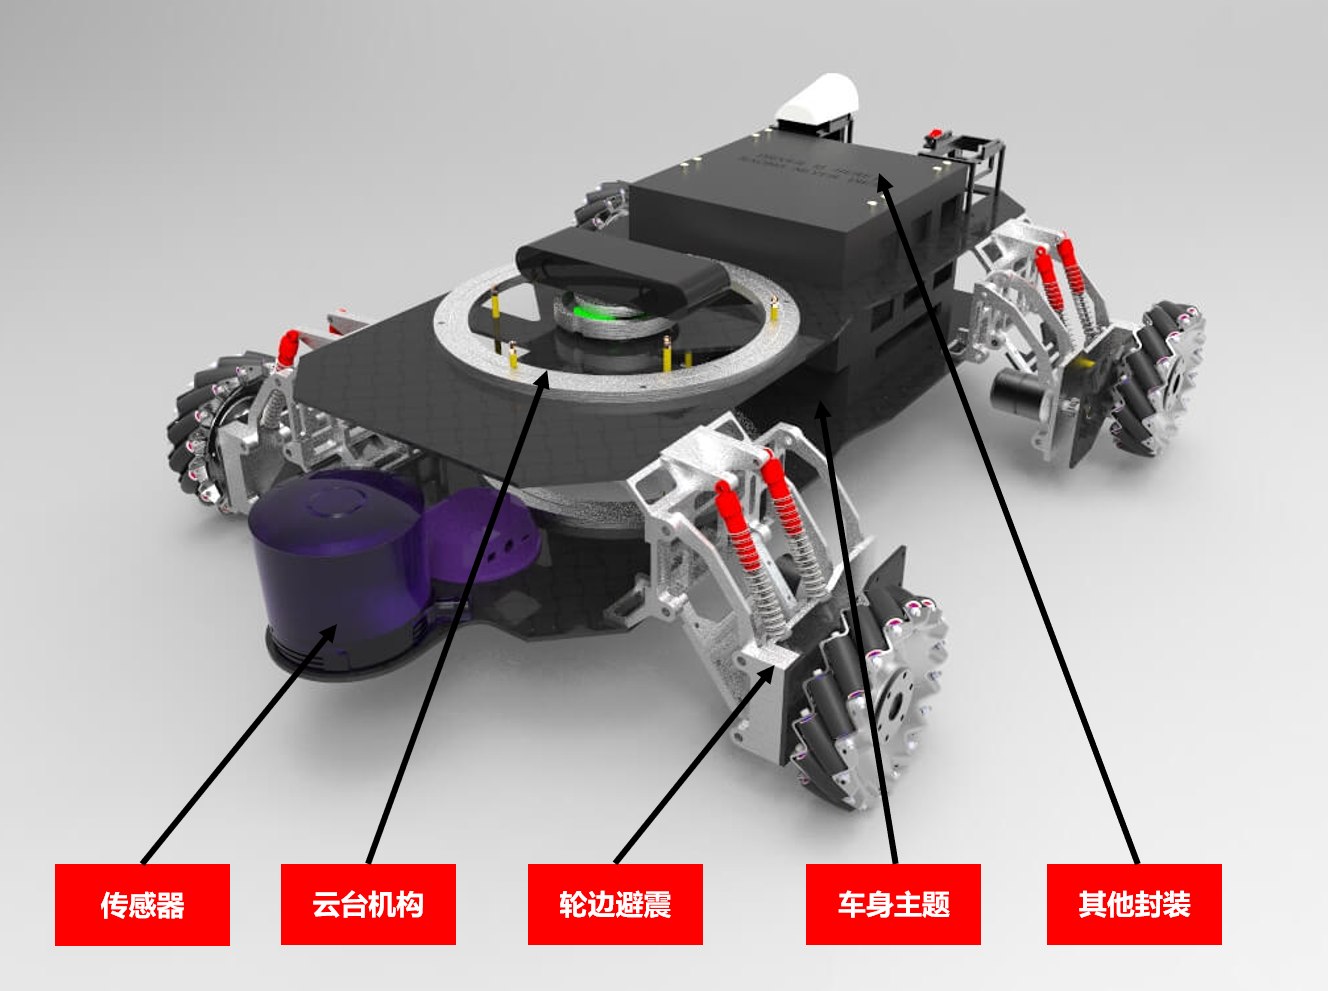
\includegraphics[width = 0.5\textwidth]{fig/overview.png}
	\caption{AtomIC平台总体示意图}
	\label{overview}
\end{figure}

\subsubsection{AtomIC平台三维渲染}

图\ref{xcsst}为AtomIC平台三维多视角的渲染图,图\ref{jdgonglu}则是在预设公路场景的渲染,如下图所示。

\begin{figure}[H]
	\centering
	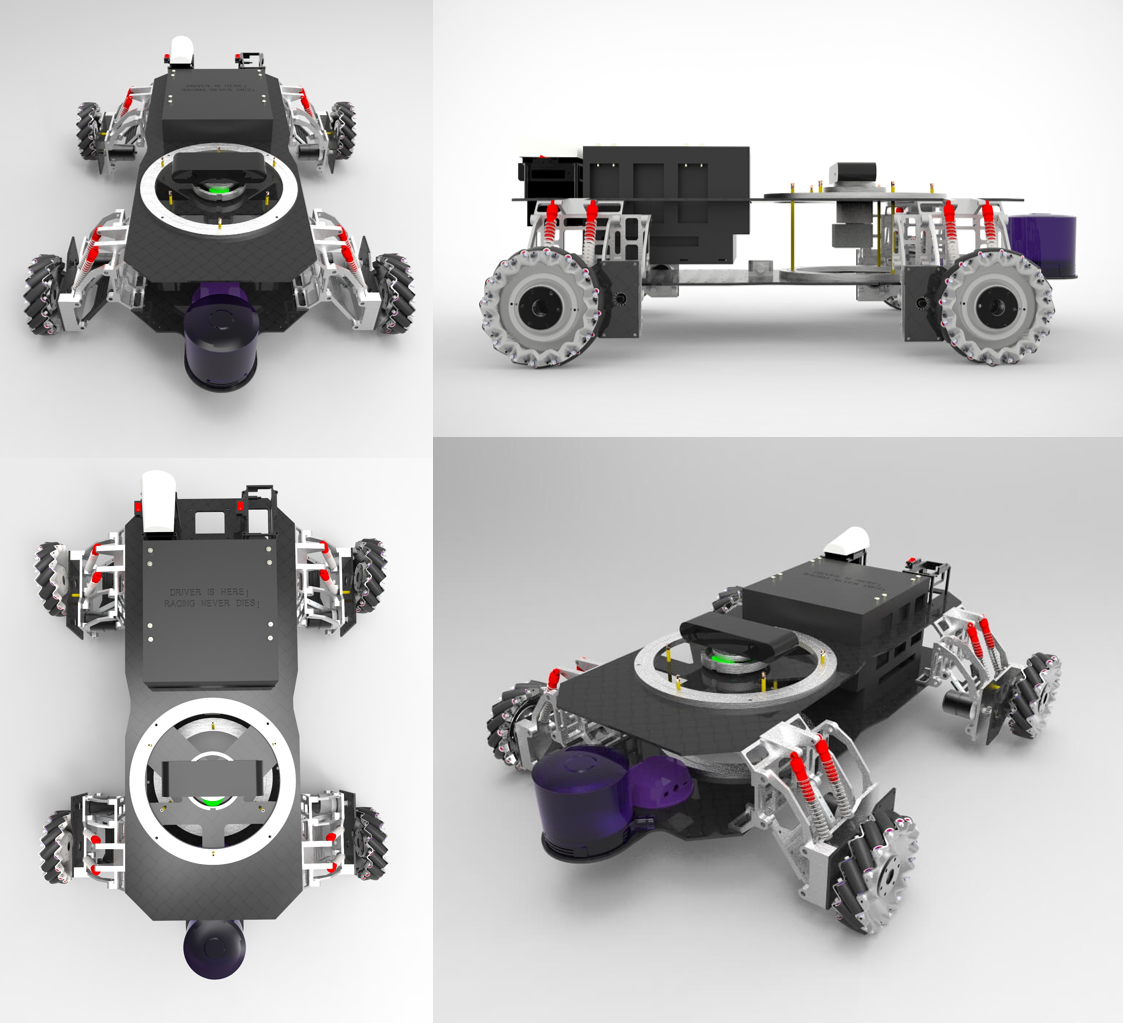
\includegraphics[width = 0.5\textwidth]{fig/xcsst.png}
	\caption{AtomIC平台渲染图}
	\label{xcsst}
\end{figure}

\begin{figure}[H]
	\centering
	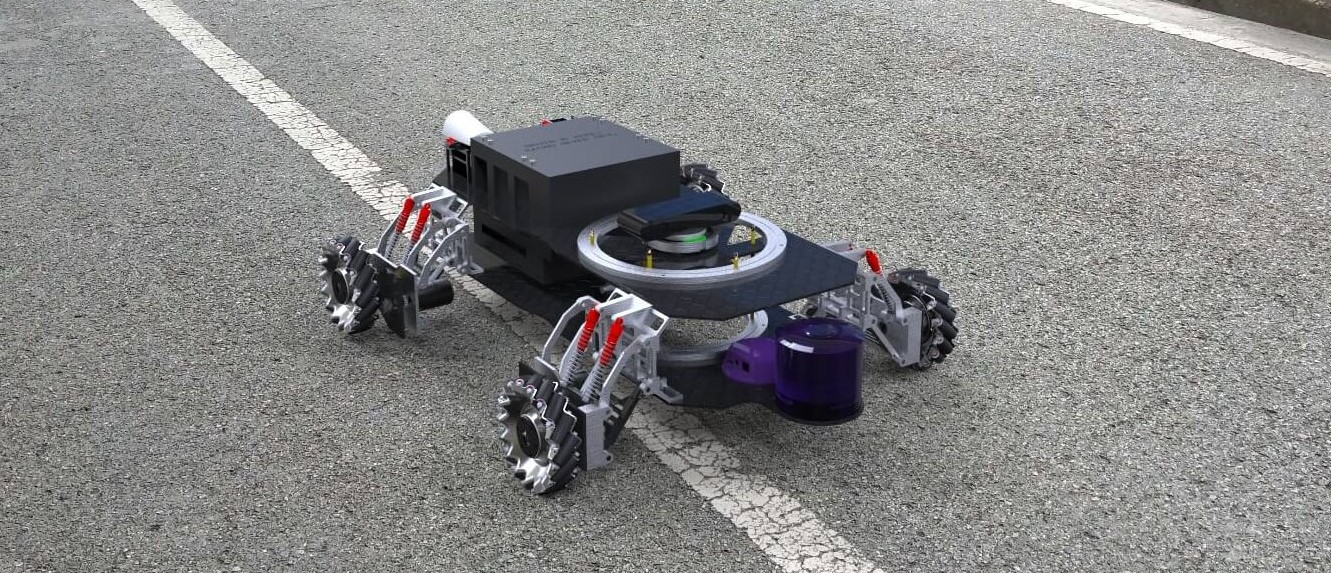
\includegraphics[width = 0.6\textwidth]{fig/jdgonglu.jpg}
	\caption{AtomIC平台在公路场景渲染图}
	\label{jdgonglu}
\end{figure}

